Data-centric governance pays dividends throughout system deployment by enabling continuous assurance systems. Without appropriate systematization, governance requirements are burdensome and likely are not adhered to over the complete system life cycle. \textbf{Governed intelligent systems require continuous assurance systems to align economic and governance requirements.}

Consider an incident where an Amazon recruiting tool systematically down-ranked female candidates whose resumes included the word ``women's'' \cite{anonymous_incident_2016}. Data-centric governance can prevent this disparate impact by surfacing the problem before deploying the system. However, even presuming the system is perfect at the time of launch, it will immediately begin to degrade as job descriptions, corporate needs, and candidate experiences continue to evolve. In time, one or more protected classes will be systematically down-ranked by the recruitment tool and Amazon would be exposed to legal and regulatory risk running into the billions of dollars. Rather than continuously monitoring and patching the recruitment system, Amazon terminated the screening program. Most, if not all, intelligent system deployments are faced with similar choices of ignoring emergent system deficiencies, developing an ongoing governance program, or terminating the deployment. The graveyard of failed AI deployments is full of projects that failed to develop assurance systems.

\highlight{
    \textbf{Can I just buy an AI system and let the vendor figure governance out?}

    Almost. As we have previously shown, a system that is not governed via data is not one that is functionally governed. So if the vendor has a comprehensive suite of tools for governing their deployments, the data and dashboards they develop should be available to their customers. If they cannot provide this information, then they likely don't have these systems and you are assuming unknowable risks.

    \takeaway{Do not buy any intelligent system without a means of continuously assessing its performance.}}

While there currently is no comprehensive solution providing data-centric governance as a service, there are several products and services providing elements of continuous assurance from the perspective of the solution team. These systems can often be deployed in support of data-centric governance with appropriate accommodation for the previously detailed principles.

\subsection{Current Systems}

While thousands of companies, consultancies, and auditors are developing tools and processes implementing governance requirements, the post-deployment governance of a system is often realized as the responsibility of the solution team rather than the verification team. Solution teams know model performance degrades through time so they monitor and improve the deployment in response to emerging changes. The associated ``model monitoring'' systems have been built with a variety of features meeting the needs of the solution team, specifically.

\begin{figure}[ht]
    \centering
    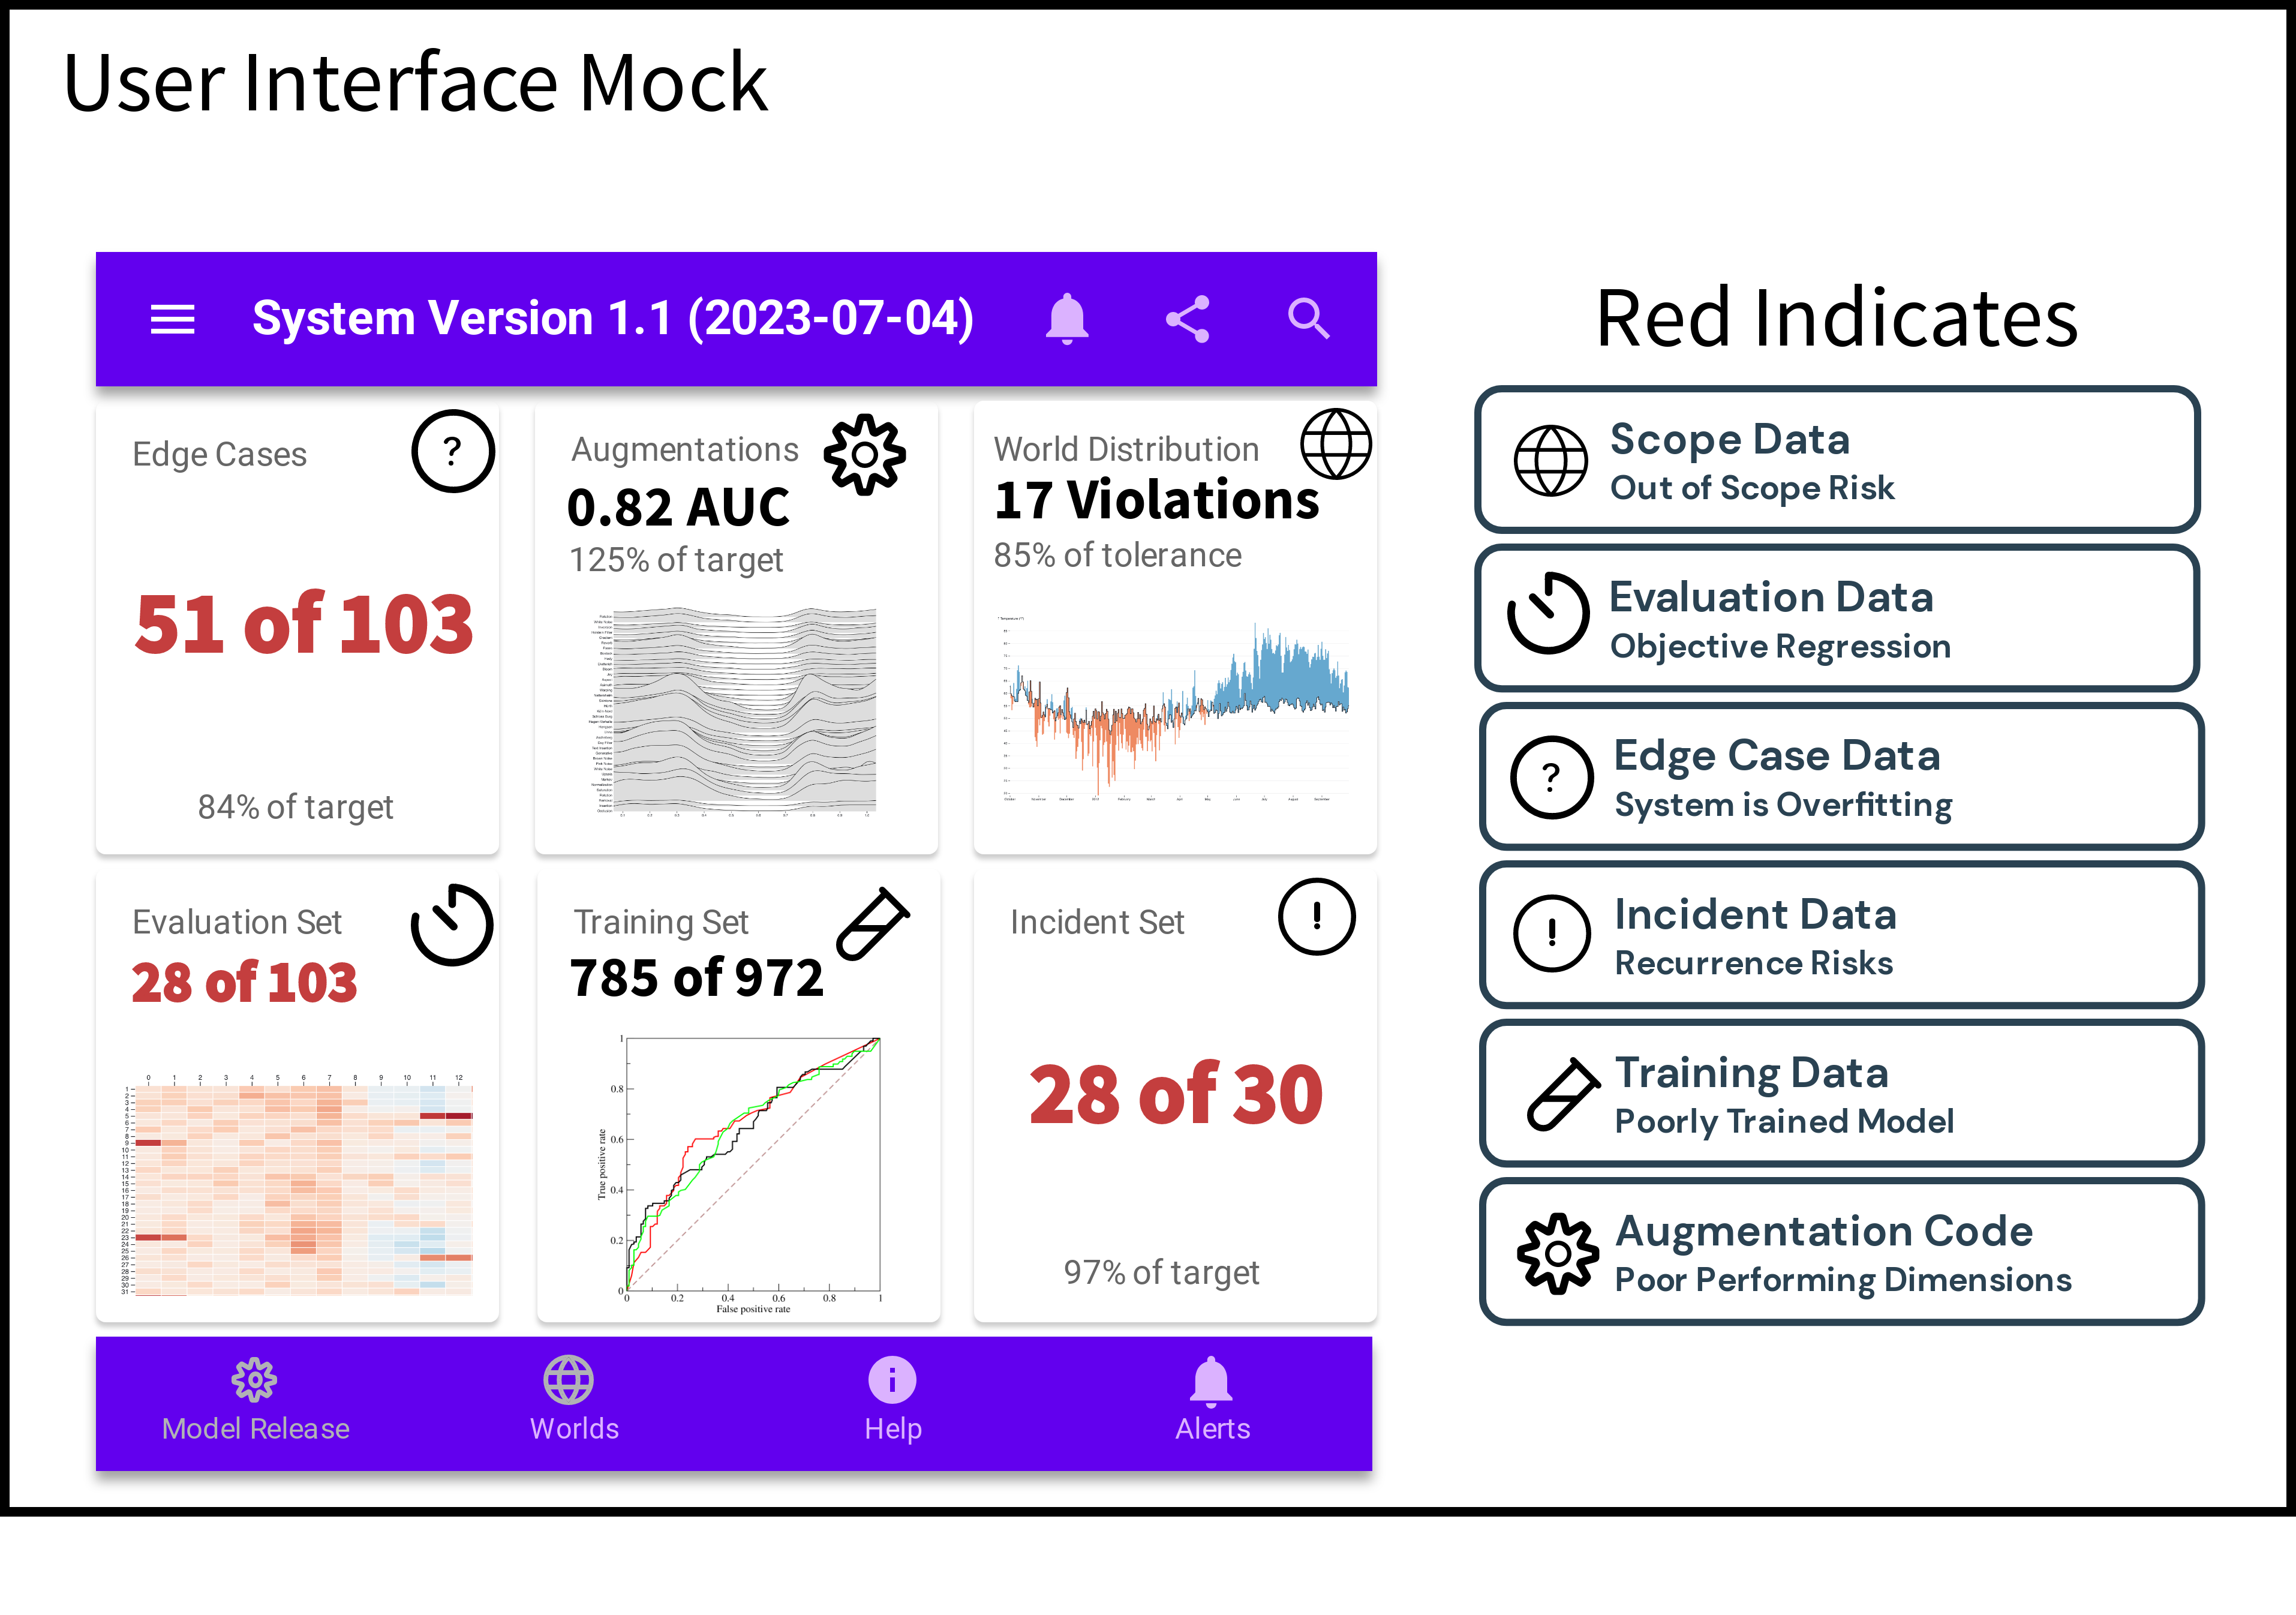
\includegraphics[width=\textwidth]{images/PenpotMock3.png}
    \caption{A high-level mockup showing a user interface for evaluating the current state of intelligent system governance. Clockwise from the upper left the panels include the current state of performance across a collection of edge cases, performance across a collection of augmentations, whether the current inputs to the system conform to the distribution assumptions of the system, the number of incidents that are prevented by the currently deployed system, the performance on the training data, and the evaluation criteria summary. Each of these panels provide humans with a capacity to oversee the performance and evolution of the system.}
    \label{fig:mock}
\end{figure}

Data-centric governance involves additional controls and procedures on top of model monitoring systems. Where a comprehensive user interface as given by Figure \ref{fig:mock} does not currently exist, the core features enabling the engineering of the user interface exist across a collection of open source and commercial offerings. The core features include:

\begin{itemize}
    \item Systems for capturing data
    \item Systems for processing data
    \item Visual interfaces
    \item Continuous Integration/Continuous Delivery (CI/CD)
\end{itemize}

We explore each of these features in turn.

% These features can be delivered as either open source solutions wherein the governance program can freely extend the software for their purposes, or via Software as a service (SaaS) offerings that provide managed infrastructure.

\textbf{Systems for capturing data.}

Computing has moved through several epochs in the distribution and maintenance of software. Initially, software could not be updated in computer systems because the hardware hard-coded the software in its physical realization. Subsequently, software could be periodically updated via physical media (e.g., punchcards or discs). Finally, software transitioned to a perpetual maintenance cycle where new versions are continually released in response to security vulnerabilities or to remain feature-competitive. The next stage in software maintenance that is informed by the needs of machine learning-based systems is to include data logging and collection.

For cloud-hosted intelligent systems, capturing live data is typically a simple matter of turning on the system's logging feature. Products that do not necessarily require a constant cloud connection regardless often ship with one for the purpose of constantly improving performance. For example, Tesla vehicles produce a variety of sensor data that is uploaded to Tesla company servers. When connectivity to the cloud is not possible, many intelligent systems have a version of the ``black boxes'' found in commercial aircraft. If these systems were not functional requirements of the final deployment, they had to have been produced during solution engineering in order to iteratively improve the solution. Thus, while not all deployed systems have the ability to collect data from the field, the absence of such systems is often a choice driven by privacy concerns or solution cost rather than a technical capacity to collect data.

\textbf{Systems for processing data.}

``DataOps'' is a rapidly expanding field of practice that aims to improve the quality, speed, and collaboration of data processes. Many startups have developed DataOps solutions for specific data types (e.g., images, video, autonomous driving, etc.) making it faster to apply human labels and programmatically process data (example in Figure \ref{fig:appen}). After the data is collected and prepared, it can be connected to simulation environments for the intelligent system. For example, NIST's Dioptra \cite{national_institute_of_standards_and_technology_what_2022} as shown in Figure \ref{fig:testbed} and Seldon Core \cite{seldon_core_seldon_2022,van_looveren_alibi_2022} give highly scalable ways to run models. All companies producing machine learning-based systems have either installed systems like these, or produced their own in house variants, during the solution engineering process.

\begin{figure}[ht]
    \centering
    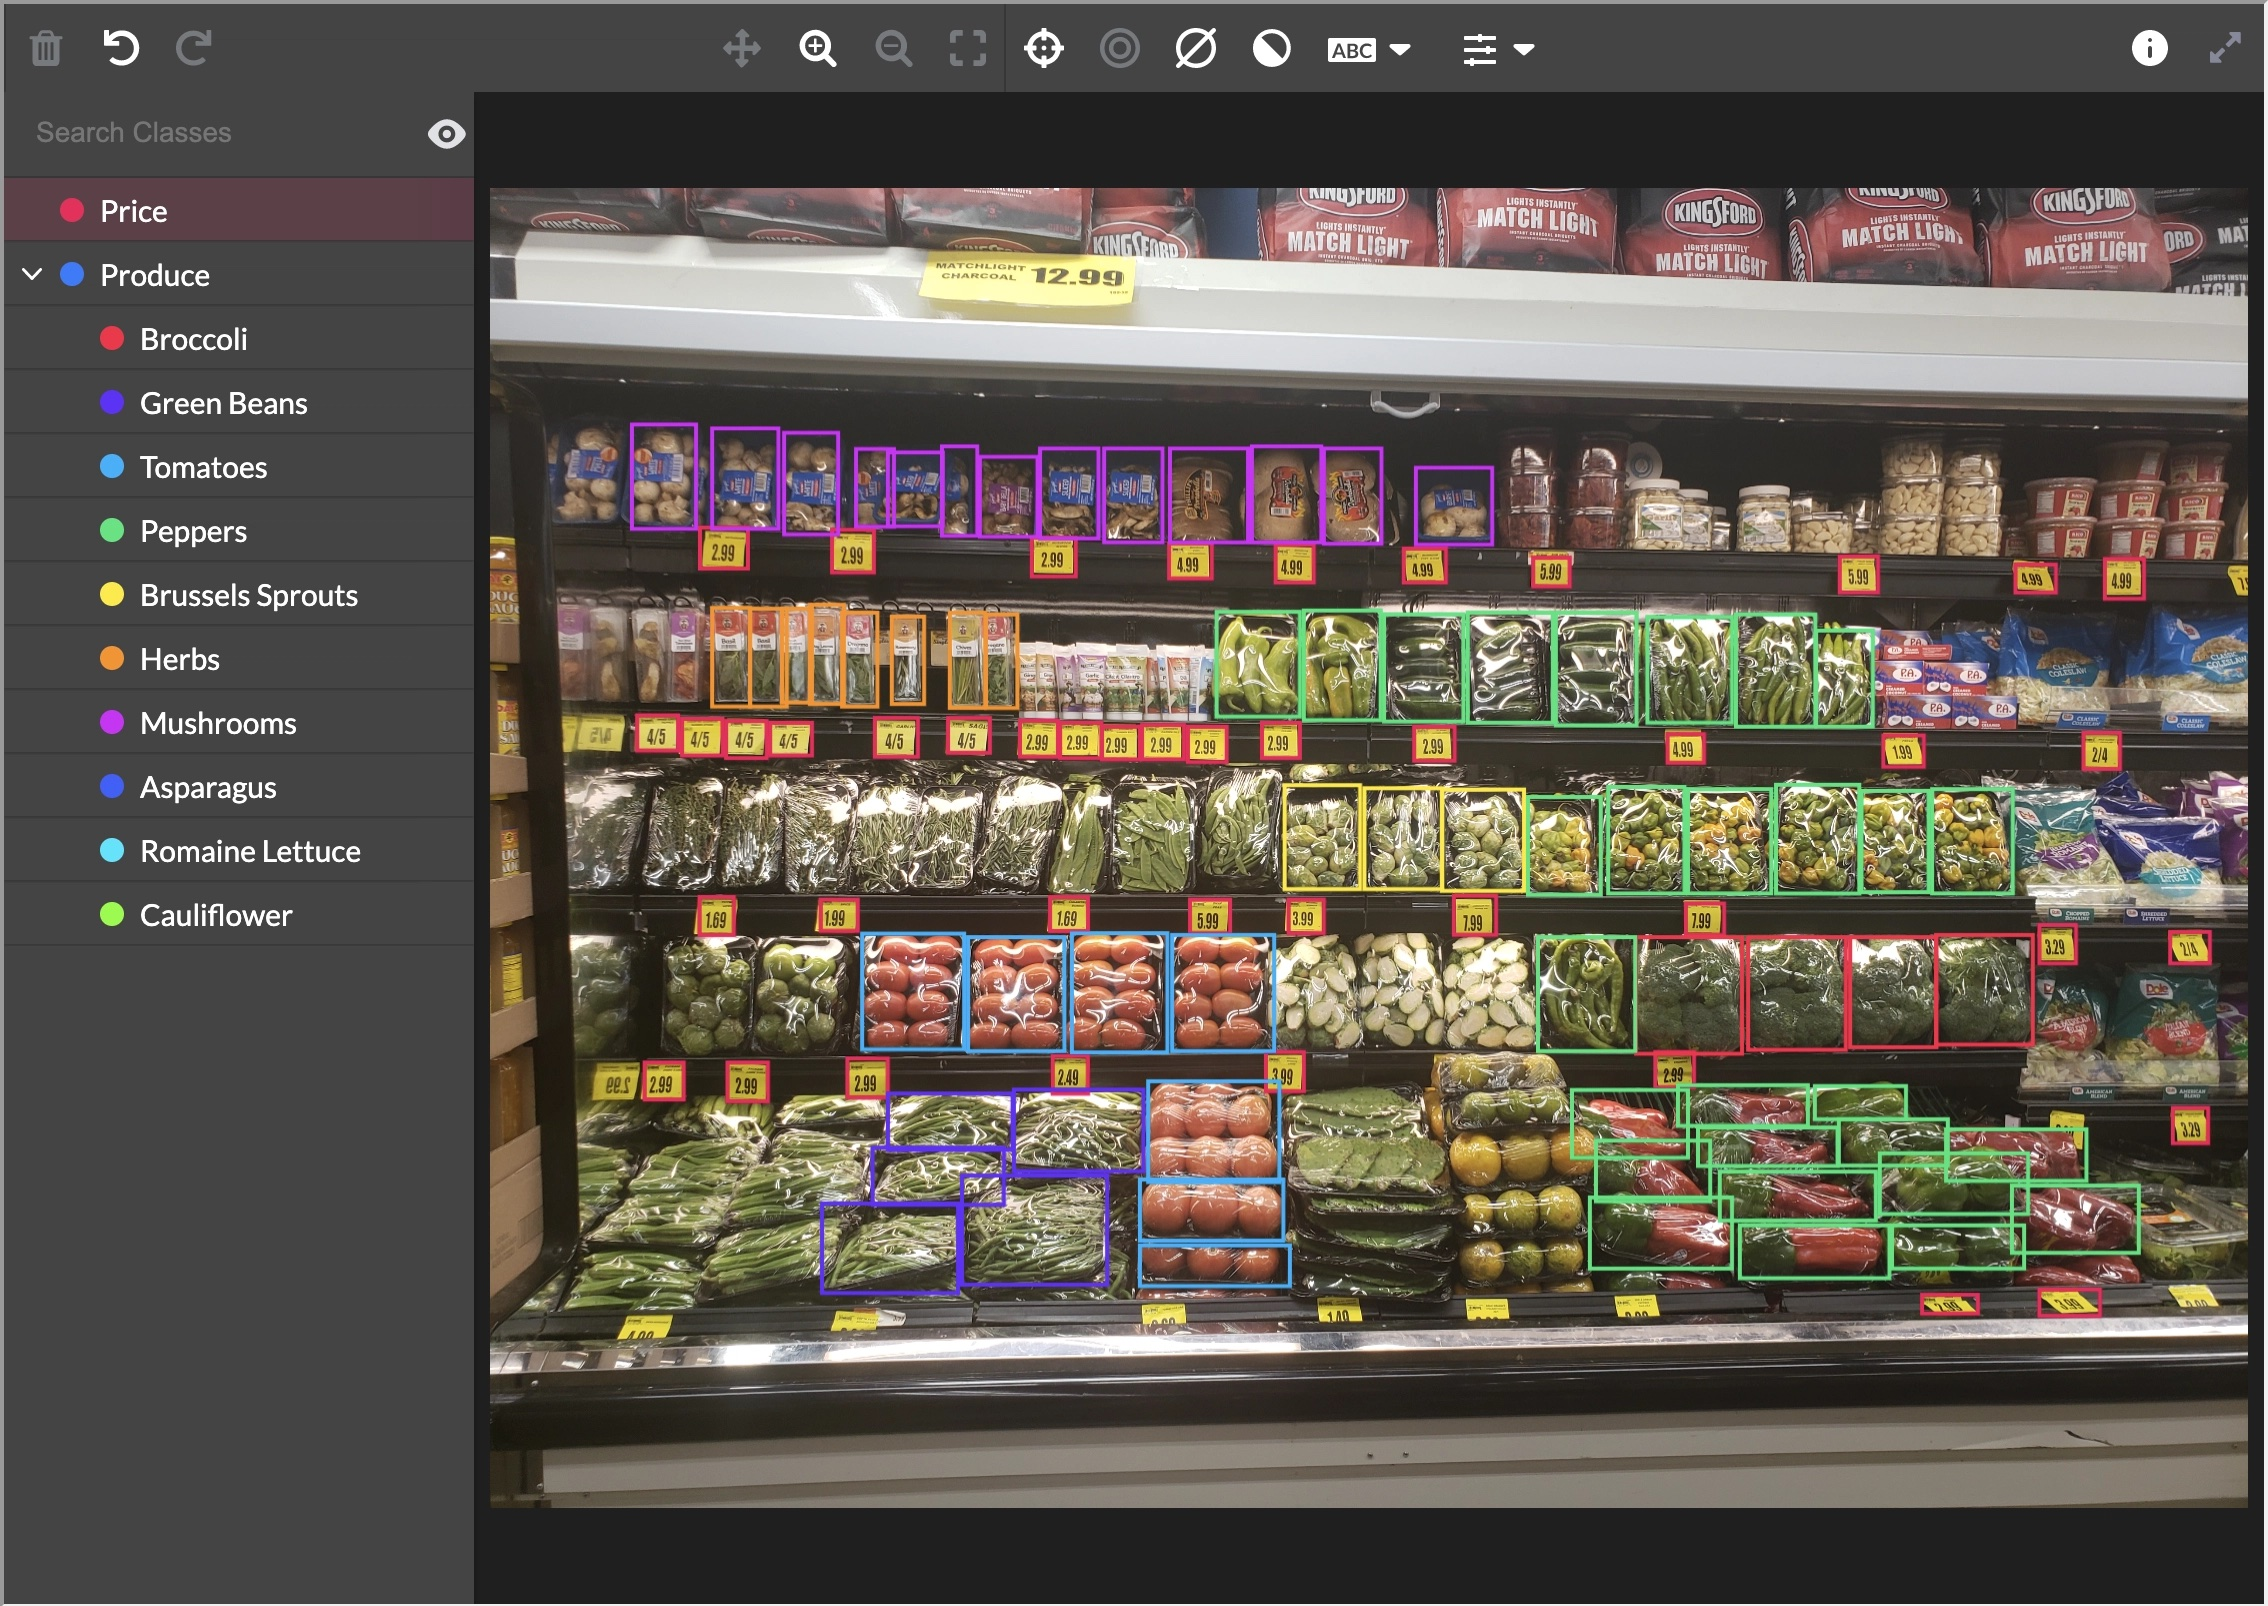
\includegraphics[width=0.7\textwidth]{images/appen.jpg}
    \caption{An example object detection user interface for examining and applying labels to an image. From the marketing page of Appen \cite{appen_launch_2022}.}
    \label{fig:appen}
\end{figure}

\begin{figure}[ht]
    \centering
    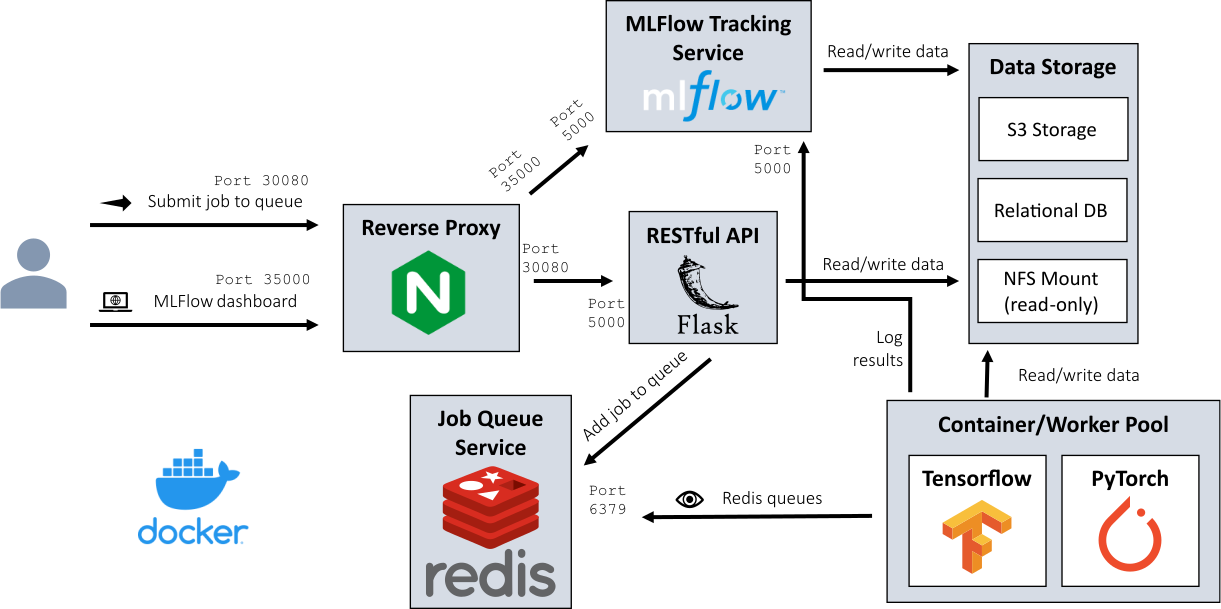
\includegraphics[width=0.7\textwidth]{images/testbed-architecture.png}
    \caption{The NIST Dioptra architecture is an open source solution for running machine learning-based models against data. It combines several open source solutions collected to supporting fast and scalable inference. From \cite{national_institute_of_standards_and_technology_what_2022}}
    \label{fig:testbed}
\end{figure}

\textbf{Visual interfaces.}

A well-implemented system will seldom need human intervention, but a well-governed one provides systems to support human analysis when governance violations are detected. For instance, in speech recognition systems environmental noise (e.g., an unusual air conditioning system) can sometimes prevent the normal operation of the system. When these cases arise the task of debugging is similar to describing an intermittent noise to an auto mechanic. No amount of human effort at mimicking mechanical clunking sounds will be as useful as providing an analytic user interface.

\begin{figure}[ht]
    \centering
    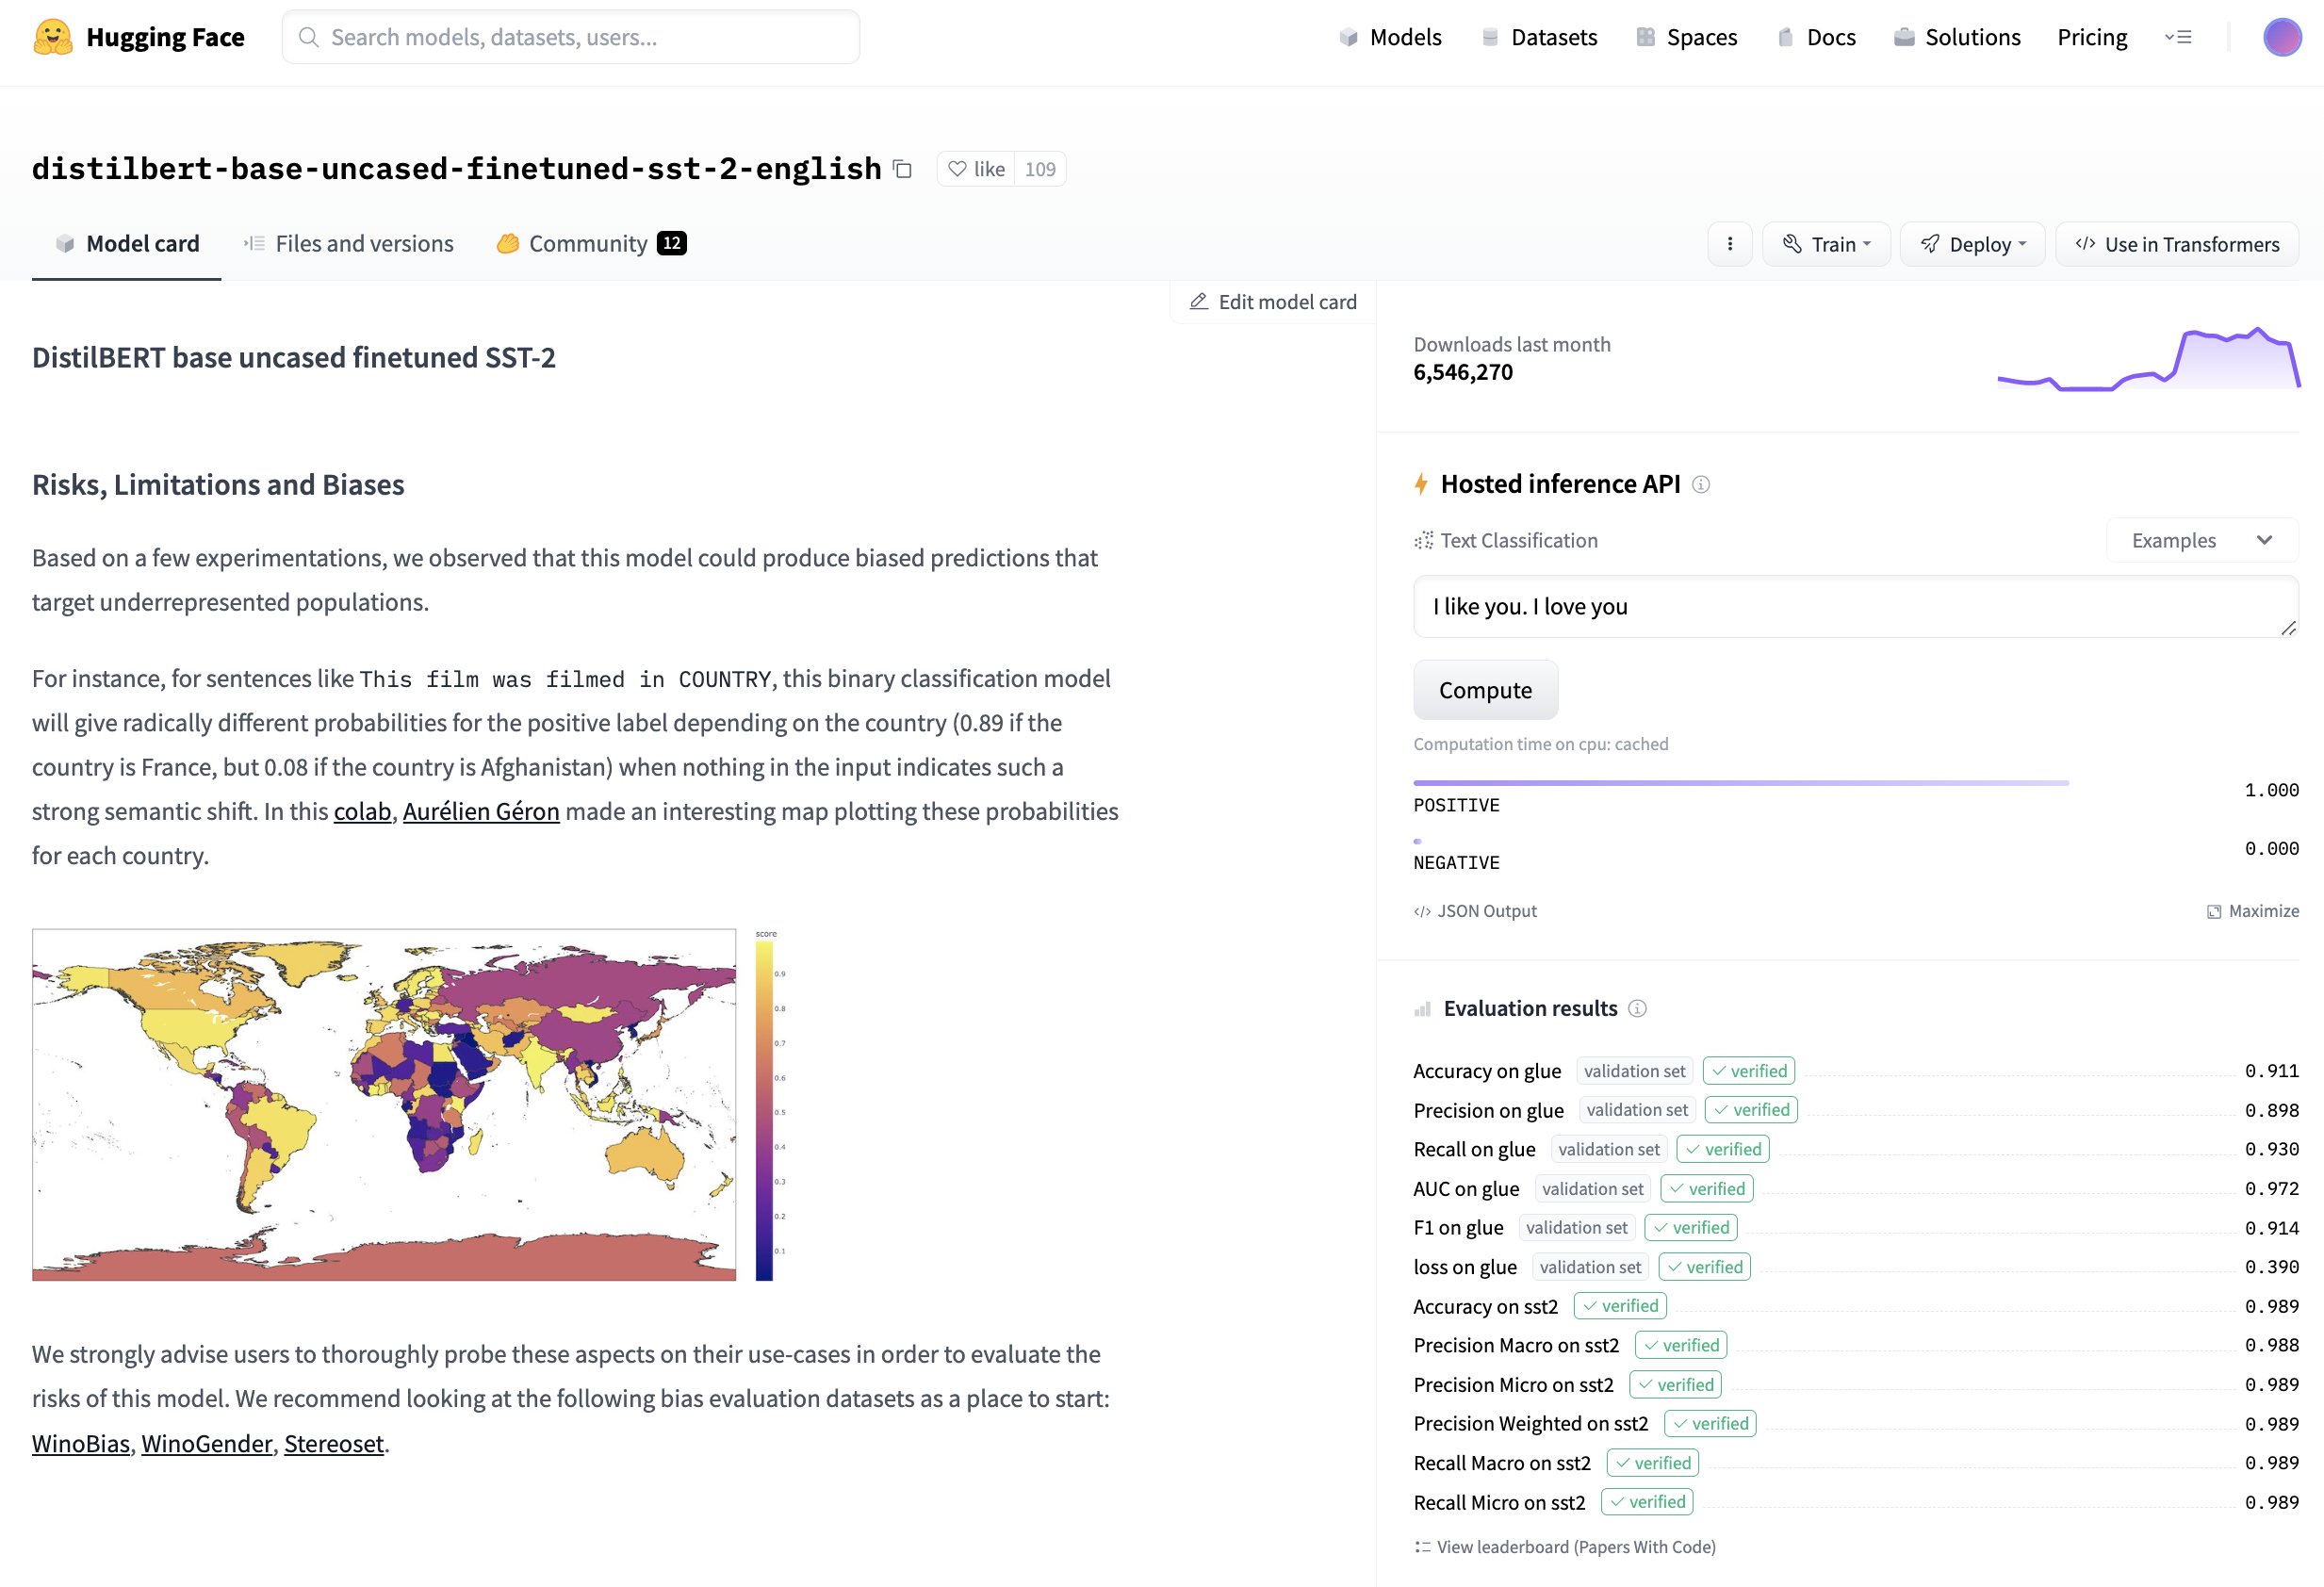
\includegraphics[width=0.8\textwidth]{images/huggingface.png}
    \caption{A model page for a language model as hosted by Hugging Face \cite{hugging_face_distilbert-base-uncased-finetuned-sst-2-english_2022}. The model can be run interactively on the page and deployed to the cloud by all visitors to the website since the model is open source. The left column provides documentation on the risks, limitations, and biases of the model, but no formal and comprehensive evaluation of the identified bias properties are provided in the dataset evaluation listing of the lower right. Understanding the biases of the model is left as an exercise to the developer making use of the model. Instead, flat performance properties like accuracy and F1 scores are presented and verified by Hugging Face staff. Given the model has been downloaded more than 6 million times, it is likely that the vast majority of model deployers have not engaged in any sort of formal governance program. Note: all the contents of the page are found on the Hugging Face website, but we have deleted some contents so all the elements in the screen capture will be rendered together.}
    \label{fig:huggingface}
\end{figure}

The model sharing and deployment company Hugging Face in one of their language models (see Figure \ref{fig:huggingface}) indicates the model presents significant biases but does not formally evaluate those biases for the community. Instead, they provide a series of top level performance properties. Model monitoring companies close the gap between data evaluation and human oversight by incorporating visual analytic user interfaces into the data logging functionality. These include Neptune.ai, Arize, WhyLabs, Grafana+Prometheus, Evidently, Qualdo, Fiddler, Amazon Sagemaker, Censius, ArthurAI, New Relic, Aporia, TruEra, Gantry, and likely others in this quickly expanding market space (see: \cite{czakon_best_2021} for a rundown).

These systems are essentially data science platforms -- they support a person exploring data as it is streaming in. What they don't do without additional effort is codify requirements in such a way that they can be checked automatically and continuously. While it is possible to continually staff a data science project with personnel applying governance requirements, the value of data-centric governance is the formalization of the monitoring activity so that people do not continuously need to watch the data as it flows in.

% \begin{figure}[ht]
% \centering
% \includegraphics[width=\textwidth]{images/time_series_light_theme_sized.png}
% \caption{todo. From \cite{grafana_labs_grafana_2022}}
% \label{fig:grafana}
% \end{figure}

\textbf{Continuous Integration/Continuous Delivery (CI/CD).}

The final system of continuous assurance is one that wraps the governance program in software systems that continuously check for compliance with requirements. Should those requirements be violated, then the system can either automatically move to a fail safe mode (typically this means shutting down) or alert humans to begin evaluating the system for potential safety and fairness issues.

Most software today is developed with systems for continuous integration (i.e., systems that continuously test for new failures or ``regressions'') and continuous delivery (i.e., systems for the deployment of a model into the real world). For instance, the developer operations (DevOps) platform GitLab provides the ability to integrate, test, and deploy software updates as shown in Figure \ref{fig:gitlab}. Seldon Core similarly provides systems shown in Figure \ref{fig:seldon} supporting humans making the decision of whether a model should be deployed after reviewing the system performance as reported in testing.

\begin{figure}[ht]
    \centering
    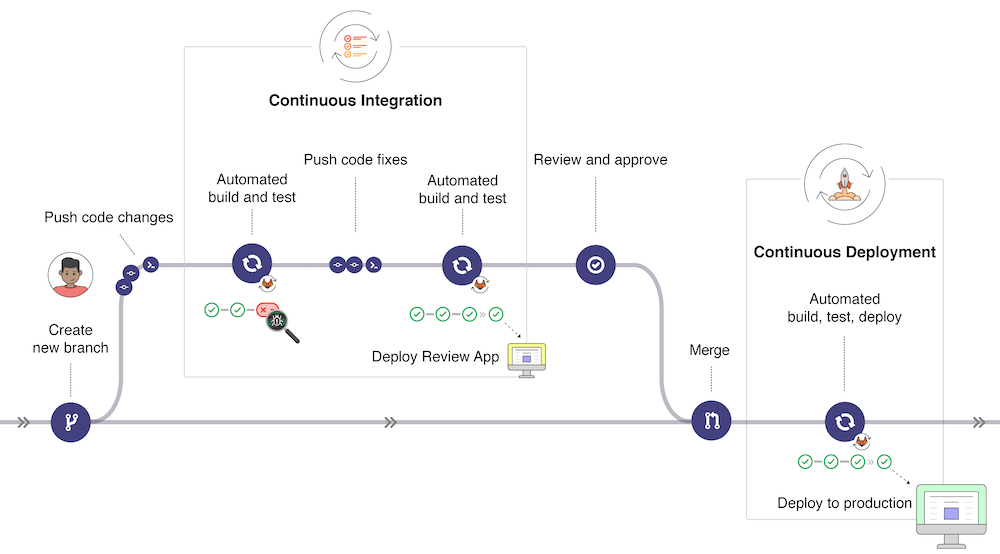
\includegraphics[width=0.7\textwidth]{images/gitlab_workflow_example_11_9.png}
    \caption{Continuous integration and delivery processes as supported by the DevOps company GitLab. The process begins with a developer creating a new version of the code, which when pushed to the GitLab server triggers a cycle of automated testing and deploying fixes to any failing tests. When the tests pass and are approved, they then move to the delivery process where additional tests are run by GitLab before the system automatically deploys to the world as the ``production'' version of the system. From \cite{gitlab_cicd_2022}}
    \label{fig:gitlab}
\end{figure}

\begin{figure}[ht]
    \centering
    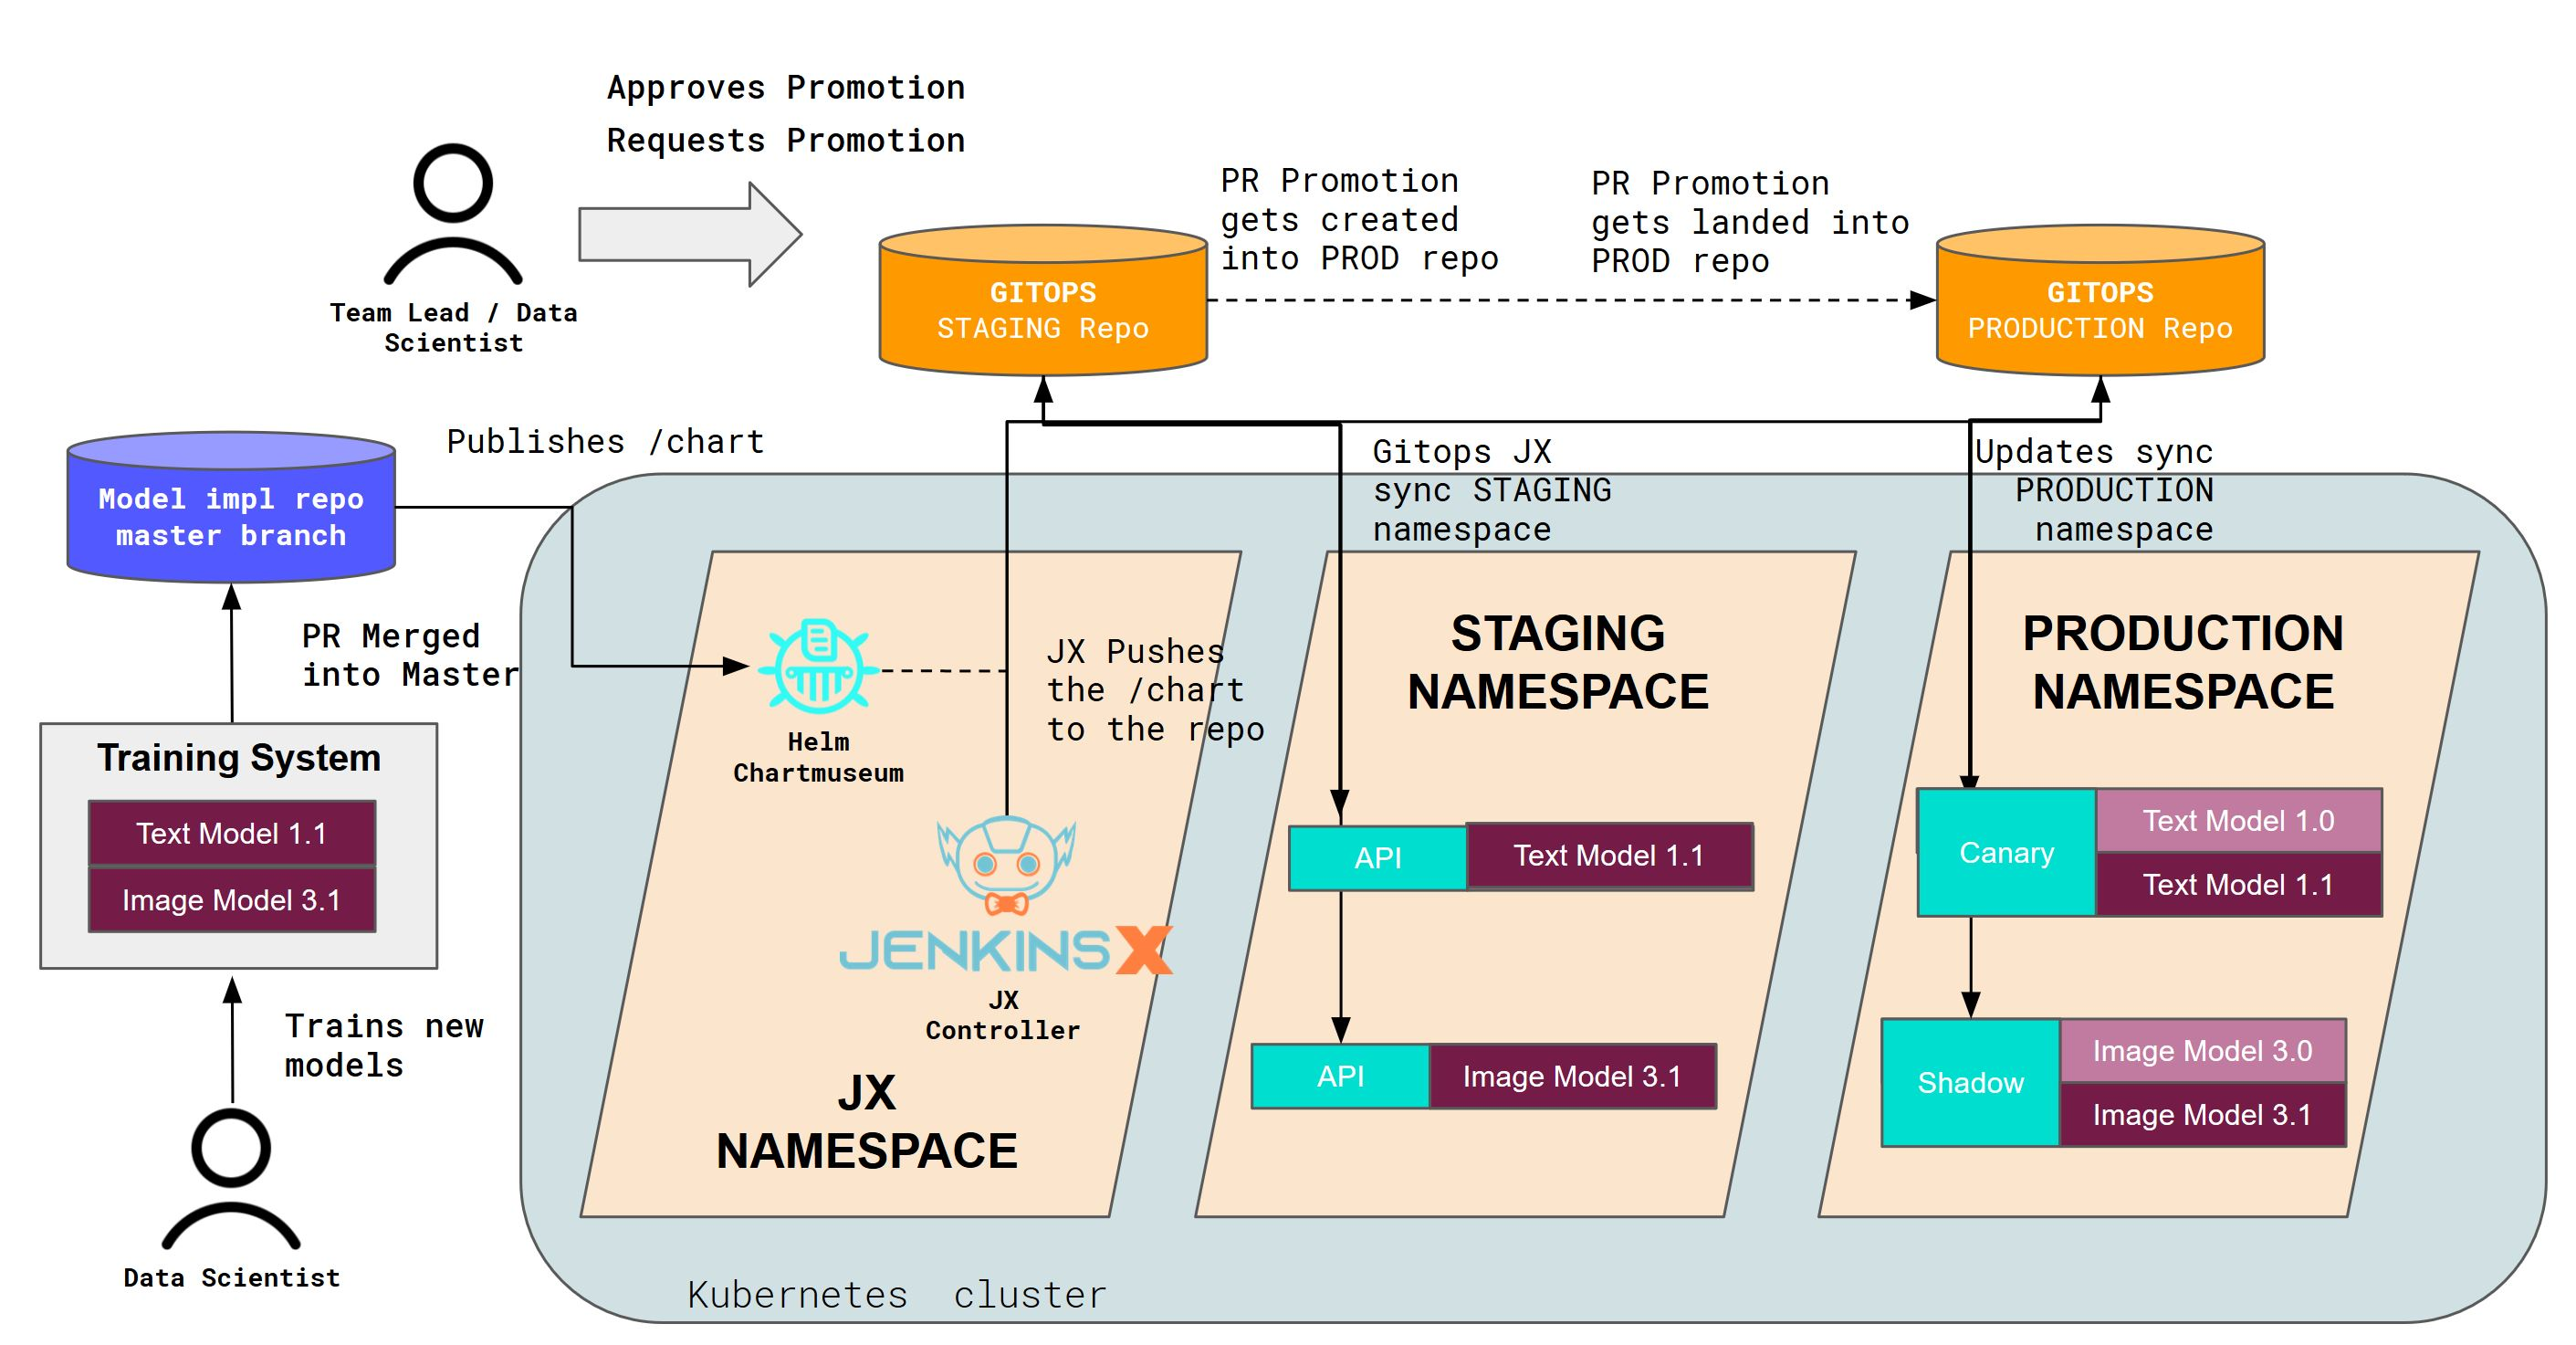
\includegraphics[width=0.7\textwidth]{images/cicd-seldon.jpeg}
    \caption{Seldon Core's model-centric view of continuous integration and delivery. Like GitLab in Figure \ref{fig:gitlab}, the process begins with a developer (here a data scientist) updating the implementation, which then goes into a scalable computing environment known as a ``Kubernetes cluster.'' The scalable computing environment then runs tests and an approver can decide whether the update goes to a staging environment for further testing and/or the live production environment. As a data-centered practice, the system has multiple versions deployed simultaneously so each can be statistically compared in their live performance. \cite{seldon_core_seldon_2022}}
    \label{fig:seldon}
\end{figure}


% \textbf{Cloud Systems.}

% Most commonly monitoring systems presume the intelligent system is cloud hosted to enable comprehensive logging and the presentation of a user interface showing current system properties.


